\section{Encoding Attribute Sets}
\label{sec:flextag_encoding} 
The simplest way to encode a set of attributes is a bitmask with one
bit for each attribute, at the expense of large tags.  In this
section, we present a concise encoding that uses multiple smaller
bitmasks on different subsets of attributes, at the expense of
slightly larger rule tables.  We also present an algorithm for
computing the concise encoding.

\subsection{Strawman: Bitmask Tags}

We will now present a strawman tagging scheme which always achieves optimum switch memory usage by using wildcard matches.
If there are $N$ possible attributes to encode in a tag, construct a tag of length $N$: 
the $i^{th}$ bit corresponds to the $i^{th}$ attribute. When the packet is classified
and the tag is attached, the $i^{th}$ bit is set to 1 if the $i^{th}$ attribute
is present for that flow, and 0 if it is not. As a result, if we wish to test for
the presence of attribute $x$, we need only check that $x$'s bit is 1 in the
tag, rather than exact matching on every tag that contains
$x$.

This approach is a strawman because the tag is of width $N$, and $N$ can be quite large.
Although we criticized flat tagging for using too much switch memory, 
flat tagging only needed tag width logarithmic in the number FECs. We have just traded an extreme in memory
usage for an extreme in tag width. It would be ideal to find some middle ground.
In general, any tagging scheme must simultaneously consider three different metrics:

\begin{enumerate}
\item \textbf{Tag Width:} Tags should not be too wide, to avoid wasting packet-header space.
Tags should be able to either be inserted into small repurposed header fields or contribute little size to custom packet headers. 
\item \textbf{Switch Memory:} The amount of memory required to decode attributes from any tag should be able to easily fit in modern commodity switches rule tables.
\item \textbf{Churn:} Normal network events should not cause the encoding scheme to undergo too many changes.
\end{enumerate}
%It is these metrics by which we will evaluate our solution.
%%%%%%%%%%%%%%%%%%%%%%%%%%%


%To understand the problem, let us consider a
%simple example for the case of attaching lists of anycast hosts to a packet. Say
%that there is a local area network with five hosts $H = \{h_1, h_2, h_3, h_4,
%h_5\}$, and each packet that arrives will be classified as anycasting to one of
%four possible host sets: $s_1 = \{h_1, h_2\}$, $s_2 = \{h_1, h_2, h_3\}$, $s_3 =
%\{h_1, h_3\}$, or $s_4 = \{h_3, h_4, h_5\}$. In a flat tagging solution to this
%problem, each unique set will be assigned a single tag, and thus a packet which
%can be forwarded to the $i^{th}$ set will receive the $i^{th}$ tag. Now, for an
%intermediate switch to determine, using exact tag matches, if a packet can be
%forwarded to host $h_1$, it must check whether the packet has been assigned to
%$s_1, s_2,$ or $s_3$. The number of entries required is proportional to the
%number of sets which contain $h_1$, in this case 3. In the worst case $h_1$
%would be a member of almost every group, and testing for $h_1$ would required a
%number of checks linear in the number of tags. 

\begin{figure}[t!] \begin{minipage}{1\linewidth}
\begin{subfigure}[b]{0.96\linewidth} 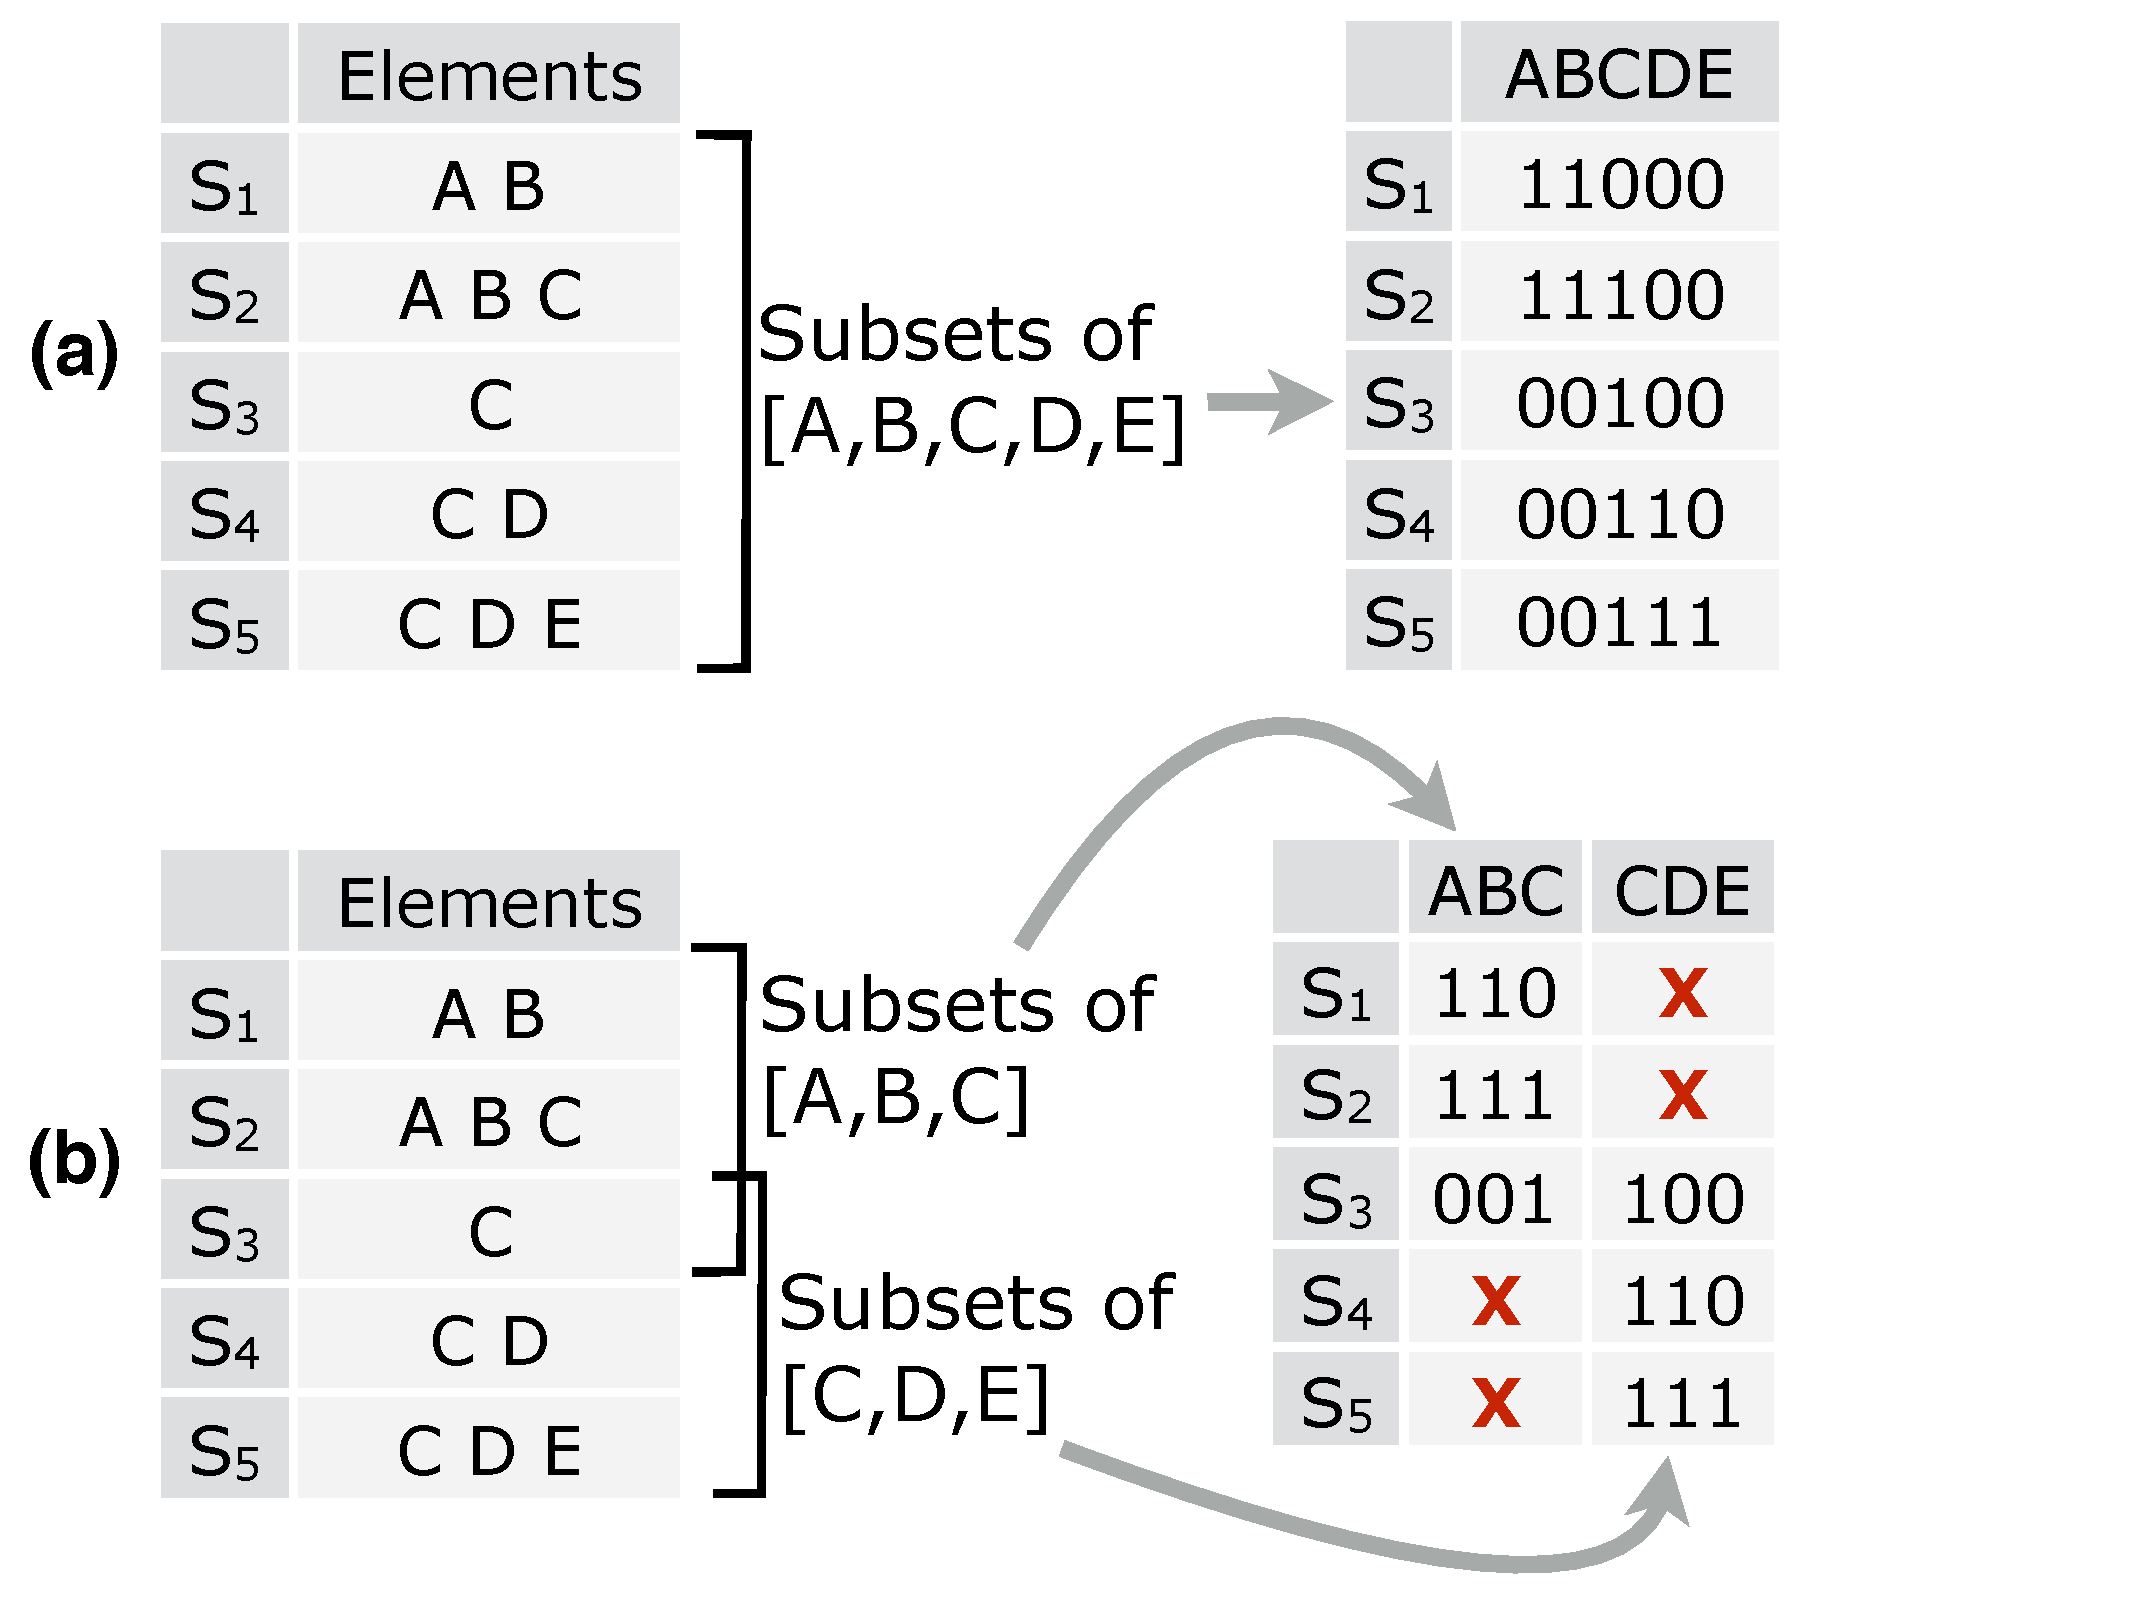
\includegraphics[trim={0 0 5.5cm 0}, clip,
width=\linewidth]{figures/masking} \end{subfigure}
\begin{subfigure}[c]{0.96\linewidth} 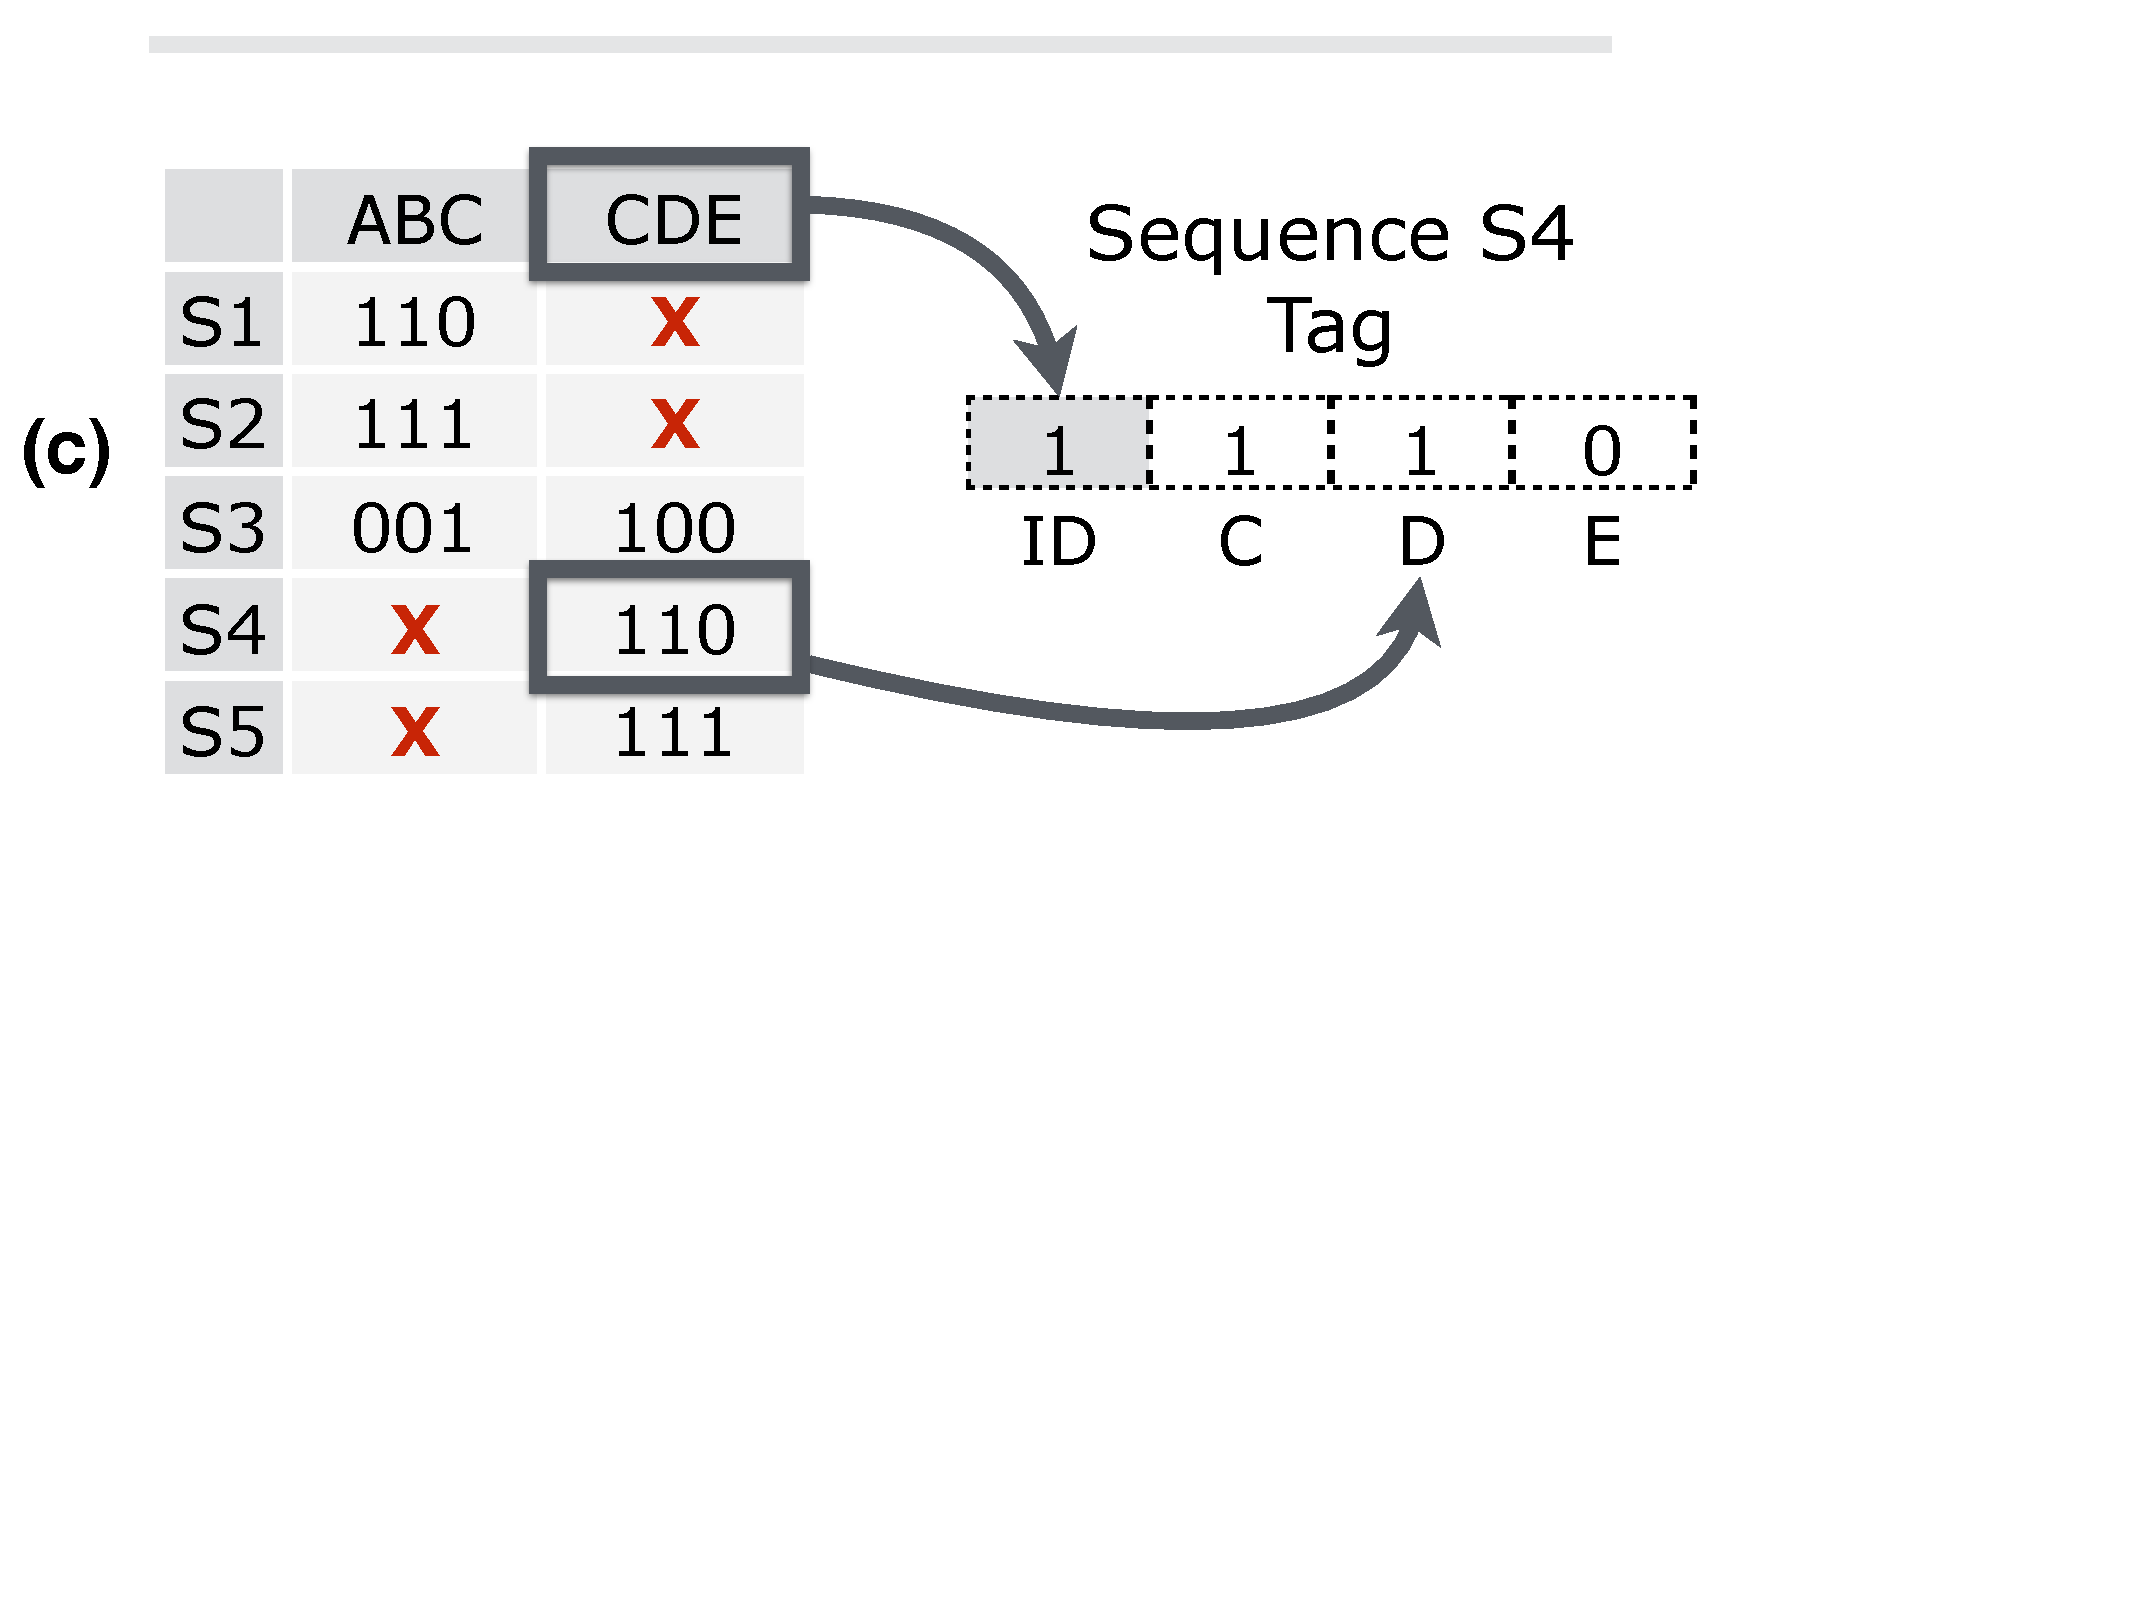
\includegraphics[trim={0 13cm 5.5cm 0},
clip, width=\linewidth]{figures/making_metadata} \end{subfigure} \end{minipage}
\caption{Two different ways to recover attribute sets.
In (a), the sets are recovered by masking over $[A,B,C,D,E]$. In (b), the sets
are recovered by masking over either superset $[A,B,C]$ or set $[C,D,E]$. An $X$
denotes that the set cannot be fully recovered by masking over the given set.
(c) shows how the matrix in (b) can be mapped to tags.}
\label{fig:masking} \end{figure}

\subsection{Multiple Smaller Subsets of Attributes}
\label{ssec:mset}
%%%
%%% Strawman
%%%
In the strawman solution of a simple bitmask, the tag has one bit for
each boolean attribute.  For example, Figure~\ref{fig:masking}(a)
shows multiple attribute equivalence classes ($S_1$-$S_5$) that each
correspond to a different subset of five attributes ($A$-$E$).  The
network policy determines which traffic has which attributes, and
which combinations of attributes can hold together.  For example, all
packets with attributes $A$ and $B$ true, and $C$, $D$, and $E$ false,
belong to attribute equivalence class $S_1$, and can be encoded with
the bitmask ``$11000$''.  Certain combinations of attributes may not
occur for any traffic (e.g., attributes $B$ and $D$ are never true
together, though both can be false as in $S_3$).  A single rule can
test for any combination of attributes (e.g., comparing a tag to
$\textsc{``1*1**''}$ identifies whether attributes $A$ and $C$ hold, without
caring whether $B$, $D$, or $E$ hold).  However, when the number of
attributes is large, a bitmask tag becomes quite large.

%%%
%%% Concise encoding example in the figure
%%%
Our more concise encoding identifies groups of attributes that
commonly appear together, and creates one shorter bitmask for each
such group.  In the example in Figure~\ref{fig:masking}, attributes
$A$, $B$, and $C$ commonly appear together, as do $C$, $D$, and $E$,
leading to two groups.  The right side of Figure~\ref{fig:masking}(b)
shows how each attribute equivalence class can be encoded as a bitmask
on $[A,B,C]$, $[C,D,E]$, or both.  To differentiate between the two
groups, the tag can include a one-bit group identifier (e.g., a $0$
for $[A,B,C]$ and a $1$ for $[C,D,E]$), as shown in
Figure~\ref{fig:masking}(c).  The result is a four-bit identifier
where, for example, $S_4$ with attributes $C$ and $D$ is encoded as
$1110$.

%%%
%%% Slightly larger rule table
%%%
The forwarding rules can match on attributes by considering both the
group identifier and the associated bitmask.  For example, a switch
could test for attribute $D$ by matching on (i) group $1$ and (ii) the
$D$ bit in group $1$'s bitmask.  Thus, the rule would have a match of
``$\textsc{1*1*}$".  However, some attributes appear in multiple groups, such
as attribute $C$ in the example.  The switch can use two rules to test
for $C$: (i) ``$\textsc{0**1}$'' for group $0$ and (ii) ``$\textsc{11**}$'' for group
$1$.  Thus, our encoding scheme slightly increases the forwarding
table size over the simple bitmask scheme, but only by one rule in
this example.

\subsection{Computing Concise Encodings of Sets}
\label{ssec:merge}
%%%
%%% Computing the initial groups
%%%
The tag and rule-table sizes depend on the quality of the encoding.  A
natural starting point is to have one group for each attribute
equivalence class (e.g., $[A,B]$, $[A,B,C]$, $[C]$, $[C,D]$, and
$[C,D,E]$), at the cost of a large group id.  A simple optimization is
to remove any group with attributes that are a \emph{subset} of
another group (e.g., removing $[A,B]$ and $[C]$ that are subsets of
$[A,B,C]$, and removing $[C,D]$ that is a subset of $[C,D,E]$).  In
the simple example, this heuristic results in the two groups
($[A,B,C]$ and $[C,D,E]$).  However, in larger examples, this
heuristic could still result in too many groups. Instead, we use the
set of groups ($\SS$) produced by the heuristic as an input to an
algorithm for optimizing the selection of groups.

\begin{algorithm}
\DontPrintSemicolon
\KwData{Groups $\SS$, Attribute Test Counts $\{q_k\}$, 
  Tag Width Limit, $W_{max}$, Tag Width Calculator $W()$.}
\KwResult{Groups $\SS$ with minimal rule-table size.}
\Begin{
\While{$|\SS| > 1$}{
      	$bestPair \gets (None, None)$\;
      	$bestGain\gets 0$\;
      	\For{$(s_i, s_j) \in \SS\times \SS$}{
      		$\SS_{temp} \gets (\SS-\{s_i, s_j\}) \cup \{s_i\cup s_j\}$\;
      		\If{$W(\SS_{temp}) \le W_{max}$}{
      			$gain \gets \sum_{k \in s_i\cap s_j}q_k$\;
      			\If{$gain > bestGain$}{
      				$bestGain \gets gain$\;
      				$bestPair \gets (s_i, s_j)$\;
      			}
      		}
      	}
      	\If{$bestPair = (None, None)$}{
      		\textbf{break}\;
      	}
      	$(s_a, s_b) \gets bestPair$\;
      	$\SS \gets (\SS-\{s_a, s_b\}) \cup \{s_a\cup s_b\}$\;
      }
      \textbf{return} $\SS$\;
}
\caption{Greedy Memory Minimization\label{alg:memory_min}}
\end{algorithm}

%%%
%%% Benefits of merging groups
%%%
Our algorithm iteratively merges pairs of groups, to minimize the
rule-table size while staying within some limit $W_{max}$ on the tag
size.  Suppose a switch has $q_a$ clauses that test whether attribute
$a$ is true, and the attribute appears in $k_a$ groups.  Then, the
switch would require $q_a \cdot k_a$ rules to test for that attribute.
Merging two groups can reduce the number of rules, but possibly
increase the tag size depending on the number of attributes the two
groups have in common.  Suppose $\SS = \{s_1, s_2, \dots, s_N\}$,
where group $s_i$ is a subset of attributes.  Replacing any pair of
groups $\{s_i, s_j\}$ with their union $s_i\cup s_j$ would decrease
the number of rules by $\sum_{a \in s_i\cap s_j}q_a$ because every
attribute $a$ in the intersection of the two groups would appear in
one fewer group after the merge.

%%%
%%% Greedy algorithm
%%%
We can extend this observation to a greedy algorithm that repeatedly
identifies the pair of groups to merge that maximally decreases the
number of rules without exceeding the $W_{max}$ tag size.
Algorithm~\ref{alg:memory_min} shows the pseudocode.  The algorithm
takes as input a set of attribute groups $\SS = \{s_1, s_2, \dots,
s_N\}$, the attribute test counts $\{q_k\}$, a maximum tag width
$W_{max}$, and a tag-width calculator $W()$.  The tag-width calculator
determines the number of bits in the tag, given the current set of
groups $\SS$.  We present closed-form equations for the tag-width
calculator later in \S~\ref{sec:identifiers}.

The algorithm runs for at most $N$ iterations, and for each iteration considers $N^2$ pairs of attribute groups, resulting in an overall complexity of $O(N^3)$. As presented, the tag width calculator is $O(N)$ complexity, which would result in a total complexity of $O(N^4)$, however in practice we can avoid recomputing the width from scratch and perform only a constant amount of work every iteration. 

